%!TEX root = ../../clcxsj.tex

\chapter{\cs 面向对象特性}

类(class) 是面向对象程序设计的基础与核心,封装、继承、多态(polymorphism)是面向对象程序设计的三大特征。

封装把客观事物封装成抽象的类,在类中把自己的数据和方法只让可信的类或者对象操作,对不可信的类或对象进行信息隐藏。

也就是应尽可能的把类成员变量的访问权限定为 private 或 protected ,通过属性(Property)或方法向外开放;
类的方法/函数 应尽可能的定义为 public ;
需向下继承的类成员,尽可能可以定义为 protected ;
项目内能访问的成员,尽可能定义为 internal 。

继承 (Inheritance) 是指这样一种能力:它可以使用现有类的所有功能,并在无需重新编写原来的类的情况下对这些功能进行扩展。

继承符合开闭原则。

通过继承创建的新类称为“子类”或“派生类”, 被继承的类称为“基类”、“父类”或“超类”。
继承的过程,是从一般到特殊的过程。

多态(polymorphism)是指将子对象赋值给父对象,父对象就可以根据当前赋值给它的子对象的特性以不同的方式运作。


\section{类与对象}
类是 \cs 中最基础最重要的类型,是一种将数据(字段)与对数据的操作(方法、函数以及属性等)组合在一起的数据结构。

严格地说,类分为实例类与静态类,实例类为动态创建类的实例 (instance) 提供定义,
实例也称为对象 (object)。也可以说类是定义,对象是类的实例。
静态类不能生成类的实例,在此声明,若非特别语境下,以后本书中所指的类均为实例类。

在 \cs 中类支持单继承 (inheritance),通过类继承产生派生类 (derived class), 
从而扩展和专用化基类 (base class) 。

 \cs 中所有的类均从 System.Object 继承,如果一个类只从 System.Object 类继承,
 则可以将其省略。

 \subsection{类的定义}

类的关键字为 class ,定义一个新类的方式如下:

\begin{lstlisting}
[public/internal] class ClassName [: BaseClass, Interface1,...,InterfaceN]
{
    ......
}
\end{lstlisting}

先指定类的修饰符, class 关键字后是类名称(类名称首字母一般大写),接着是要继承的基类
与需实现的接口。
之后是类的主体,它由一组位于一对大括号 ``\{'' 和 ``\}'' 之间的成员声明组成。

由于测绘行业的基本任务是提供位置服务的,点位是我们经常使用的概念,我们就对它来定义一个类 Point :

\begin{lstlisting}
public class Point : System.Object
{
    ......
}
\end{lstlisting}

上面是测量点的简单定义,关键字 class 前的 public 为访问限定符,表示访问不受限制。 
也可以为 internal ,表示该类仅限于当前程序集访问,外部程序集不能访问。
如果在 class 前不加访问修饰符,默认的访问权限为 internal 。

点名后的 ``: System.Object'' 表示 Point 类从 System.Object 类( System 为命名空间)继承。
\cs 中 System.Object 类为所有类的 根基类,如果不写类的基类,则默认从System.Object继承,
上例中 ``: System.Object'' 可以省略。

上面的代码可以简写为:
\begin{lstlisting}
public class Point
{
    ......
}
\end{lstlisting}

%%%%%%%%%%%%%%%%%%%%%%%%%%%%%%%%%%%%%%%%%%%%%%%%%%%%%%%%%%%%%%%%%%%%%%
\subsection{类的实例对象}

在 \cs 中用 new 操作符生成类的实例对象。该运算符为新的实例分配内存、
调用构造函数初始化实例,并返回对该实例的引用。

下面的语句生成两个 Point 实例对象,并将对这两个对象的引用存储在两个变量 p1 、p2 中:

\begin{lstlisting}
{
    ......
    Point p1 = new Point();
    Point p2 = new Point();
    ......
}
\end{lstlisting}

当程序执行到这段代码后边的 ``\}'' 时,将自动释放变量 p1、p2,
p1与p2所指向的内存,将由 .Net 系统自动收回。

\subsection{类的字段(Filed)}
一个类通常由两部分组成:数据与对数据的操作。字段是与类或类的实例相关的变量,
用于存储类的数据。

如上面的点 Point 类,我们可以为其定义数据成员如下:

\begin{lstlisting}
public class Point
{
    public string name;
    public string code;
    public double x;
    public double y;
    public double z;
}
\end{lstlisting}

在定义点时,点的位置属性 (x,y,z) 很容易理解,但很容易忽略点的点名与编码两个属性,
其实,测绘中往往用点名指代某个位置,点也有控制点与一般点之分,需要用编码区分点的类型,
所以点名与编码这两个字段也就很有必要。

\subsection{类字段的可访问性}

从以上点 Point 类的定义看出,每个字段的定义前都有 public ,代表着对字段的访问权限。

类的每个成员都可以关联可访问性,以控制访问该类成员的权限,默认的可访问性为private。

有六种可能的可访问性形式,如下表所示:

\begin{tabular}{|l|l|}
\hline
可访问性                 &   含义  \\
\hline
public                  &  访问不受限制   \\
protected               &  访问仅限于该类及该类的派生类  \\
internal                &  访问仅限于当前程序集  \\
protected internal      &  访问仅限于当前程序集或该类的派生类  \\
private                 &  访问仅限于包含类  \\
private protected       &  访问限于包含类或当前程序集中派生自包含类的类型。 \\
\hline
\end{tabular}

一个类可以访问自己的属性,可以通过this关键字进行引用访问,在不引起混淆的情况下,可以省略this。
this关键字指类的实例本身。

在Point类的定义 public 访问权限的数据成员后,就可以按照``实例.数据成员''进行引用了,
如下代码所示:

\begin{lstlisting}
{
    ......
    Point p1 = new Point();
    p1.name = "p1";
    p1.x = 100.0;
    p1.y = 100.0;
    p1.z = 410.0;

    Point p2 = new Point();
    p2.name = "p2";
    p2.x = 200.0;
    p2.y = 200.0;
    p2.z = 420.0;
    ......
}
\end{lstlisting}

\subsection{类的构造函数}

从上面的p1、p2的引用语句看,实际上是在给p1、p2两个点赋初值。
如果每个点都这样做的话,十分不方便。初始化实例对象更好的方法是使用构造函数。

\textbf{构造函数是函数名称与类名完全相同,且没有返回类型(即使返回类型为void也不行)的函数,
它的作用是做类的初始化工作(主要是初始化类的数据)。}

定义与使用Point类的代码如下:
\begin{lstlisting}
//在Point.cs文件中定义
public class Point : System.Object
{
    public string name;
    public string code;
    public double x;
    public double y;
    public double z;

    public Point(string name, string code, double x, double y, double z)
    {
        this.name = name;
        this.code = code;
        this.x = x;
        this.y = y;
        this.z = z;
    }
}

//在Program.cs文件中Main()函数中使用
Point p1 = new Point("p1", "", 100.0, 100.0, 410.0);
Point p2 = new Point("p2", "", 200.0, 200.0, 420.0);
\end{lstlisting}

构造函数支持重载(overload)。所谓的\textbf{函数重载} 就是函数名称相同,但函数的参数类型或参数个数不一样。
请注意,函数重载没有关注函数的返回值,只关注了函数的参数。

没有参数的构造函数称为\textbf{默认构造函数}。如果类中不定义任何构造函数,系统会为我们生成一个默认构造函数,
一旦我们定义了一个构造函数,系统就不会为我们再生成这个默认构造函数。
如果仍然要使用这个默认的构造函数,需要显式定义。

为了方便Point类的初始化,我们为Point类定义多个构造函数如下:

\begin{lstlisting}
//在Point.cs文件中定义
public class Point : System.Object
{
    public string name;
    public string code;
    public double x;
    public double y;
    public double z;

    public Point() //默认构造函数
    {
        this.name = null;
        this.code = null;
        this.x = 0;
        this.y = 0;
        this.z = 0;
    }

    public Point(double x, double y)
    {
        this.name = null;
        this.code = null;
        this.x = x;
        this.y = y;
        this.z = 0;
    }

    public Point(double x, double y, double z)
    {
        this.name = null;
        this.code = null;
        this.x = x;
        this.y = y;
        this.z = z;
    }

    public Point(string name, double x, double y)
    {
        this.name = name;
        this.code = null;
        this.x = x;
        this.y = y;
        this.z = 0;
    }

    public Point(string name, double x, double y, double z)
    {
        this.name = name;
        this.code = null;
        this.x = x;
        this.y = y;
        this.z = z;
    }

    public Point(string name, string code, double x, double y, double z)
    {
        this.name = name;
        this.code = code;
        this.x = x;
        this.y = y;
        this.z = z;
    }
}
\end{lstlisting}

注意以上构造函数中的 this 关键字不可省略, this.name 限定了name 是类中的name,
而 ``='' 后的 name 根据就近原则指的是函数参数中的name。
其含义为将参数name的值赋值给类中的name字段。

有了上面重载形式的构造函数,我们就可以多种方式生成Point类的实例了,如下代码所示:

\begin{lstlisting}
//在Program.cs文件中Main()函数中使用
Point p1 = new Point();
Point p2 = new Point(100.0, 100.0);
Point p3 = new Point(300.0, 300.0, 430.0);
Point p4 = new Point("p4",400.0, 400.0);
Point p5 = new Point("p5",500.0, 500.0, 450.0);
Point p6 = new Point("p6","001", 600.0, 600.0, 460.0);
\end{lstlisting}

构造函数只能用于new操作符生成类的实例,不能显式调用。

构造函数的访问权限一般定义为public,在某些特殊的场景中也可以定义为private。
如果定义为private,该类的new操作只能在该类的静态函数中使用,在其它类中是无法生成该类的实例。

构造函数不能被继承,但子类在其构造函数中可以使用 base 关键字进行调用。

\subsection{类的属性 (property) }

在前面的Point类中我们将各个字段定义为public访问权限,这会导致在任何能引用到类的实例的地方都能
修改类中字段的数据,很显然这不符合封装的原则。在很多情况下,我们需要对类中数据的访问与修改添加
一定的规则,比如测量行业中的坐标 (x、y) 一般情况下不能为负值。

因此,我们需将Point类中的字段访问权限定义为 private 或 protected,代码如下:

\begin{lstlisting}
//在Point.cs文件中定义
public class Point
{
    private string name;
    private string code;
    private double x;
    private double y;
    private double z;

    //此处省略掉Point的构造函数,代码如前面所示
}
\end{lstlisting}

为了支持对Point类中字段的快捷访问,\cs 中引入了\textbf{属性 (Property)}。
属性(Property) 是字段的自然扩展,是 \cs 核心语法,也是后面界面编写的核心。

属性和字段都是类的命名成员,都具有相关的类型,访问字段和属性的语法也相同。

与字段不同的是属性不存储数据。属性本质上讲是两个函数/方法(get与set),也叫做访问器 (accessor),
get代表读数据,set代表写数据,访问器指定在它们的值被读取或写入时需执行的语句。

属性的声明与字段类似,不同的是属性声明以位于定界符 \{ 和 \} 之间的一个 get 访问器和/或一个 set 访问器结束,
不是以分号结束。

Point类属性定义代码如下所示:

\begin{lstlisting}
//在Point.cs文件中定义
public class Point : System.Object
{
    private string name;
    public string Name
    {
        get{ return name;}
        set{ name = value;}
    }

    private string code;
    public string Code
    {
        get{ return code;}
        set{ code = value;}
    }

    private double x;
    public double X
    {
        get{ return x;}
        set{ x = value;}
    }

    private double y;
    public double Y
    {
        get{ return y;}
        set{ y = value;}
    }

    private double z;
    public double Z
    {
        get{ return z;}
        set{ z = value;}
    }

    //此处省略掉Point的构造函数,代码如前面所示    
}
\end{lstlisting}

同时具有 get 访问器和 set 访问器的属性是读写属性 (read-write property),
只有 get 访问器的属性是只读属性 (read-only property),
只有 set 访问器的属性是只写属性 (write-only property)。

get 访问器相当于一个具有属性类型返回值的无形参方法。
除了作为赋值的目标,当在表达式中引用属性时,将调用该属性的 get 访问器以计算该属性的值。

set 访问器相当于具有一个名为 value 的参数并且没有返回类型的方法。
当某个属性作为赋值的目标被引用,或者作为 $++$ 或 $--$ 的操作数被引用时,
将调用 set 访问器,并传入提供新值的实参。

如果属性比较简单,可以使用lambda表达式进行简写:
\begin{lstlisting}
private double x;
public double X
{
    get => x;
    set => x = value;
}
\end{lstlisting}

如果属性只有get部分,如 X 属性可以写成:
\begin{lstlisting}
private double x;
public double X => x;
\end{lstlisting}

如果属性不使用字段的话,可以简写成 get/set 形式,如 X 属性可以写成:
\begin{lstlisting}
//private double x;
public double X
{
    get;
    set;
}
\end{lstlisting}

属性的访问权限一般都定义为public,用于对外交换数据。


\subsection{类的实例方法(method)}

方法也称为函数,是类的一种行为成员,用于实现类的计算或操作。

\begin{itemize}
\item 方法的签名 (signature)

方法的签名在声明该方法的类中必须唯一。方法的签名由方法的名称、
参数类型、参数个数、返回类型、修饰符组成。

方法可以有重载形式,但必须符合重载规则。

方法的参数 (parameter) 表示传递给该方法的值或变量,参数列表可以为空;

方法还有一个返回类型 (return type),用于指定该方法的返回值类型。
如果方法没有返回值,返回类型必须定义为 void,不能不定义或省略。

\item 方法/函数的参数

参数用于向方法传数据,可以传值或传变量。
有四类参数:值参数、引用参数、输出参数和参数数组。

    \begin{itemize}
	\item 值参数 (value parameter)

    值参数用于传递值类型数据。一个值参数相当于一个局部变量,它的初始值来自于该形参传递的实参数据。
    值参数在传递时,实际上是传递值参数的一个拷贝,因此在函数内部对值参数的任何修改不会影响到传值的实参的。
    值参数在传值时可以直接传递数值。

	\item 引用参数 (reference parameter)

    引用参数可用于传递输入和输出的数据。
    在方法执行期间,引用参数与实参变量表示同一存储位置,因此为引用参数传递的实参必须是变量,
    而且必须是具有初始值的变量。

    引用参数使用 ref 修饰符声明。

    下面的交换两个变量值的代码演示了 ref 参数的用法:

\begin{lstlisting}
using System;
class Test
{
    static void Swap(ref int x, ref int y)//交换两个变量的值
     {
        int temp = x;
        x = y;
        y = temp;
    }

    static void Main()
    {
        int i = 1, j = 2; //变量i与j必须初始化
        Swap(ref i, ref j);
        Console.WriteLine("{0} {1}", i, j);  // 输出为 2 1
    }
}
\end{lstlisting}


	\item 输出参数(output parameter)

    输出参数用于函数输出计算数据值。对于输出参数来说,调用方提供的实参的初始值并不重要。
    除此之外,输出参数与引用参数类似。输出参数用 out 修饰符声明的。

    下面的代码演示 out 参数的用法:

\begin{lstlisting}
using System;
class Test
{
    static void Divide(int x, int y, out int result, out int remainder) 
    {
        result = x / y;
        remainder = x % y;
    }

    static void Main() 
    {
        Divide(10, 3, out int res, out int rem);
        Console.WriteLine("{0} {1}", res, rem); // Outputs "3 1"
    }
}
\end{lstlisting}

    第12行代码为较新式的 \cs 语法。

	\item 参数数组 (parameter array)

    参数数组允许向方法传递可变数量的实参。

    参数数组使用 params 修饰符声明。只有方法的最后一个参数才可以是参数数组,
    并且参数数组的类型必须是一维数组类型。

    System.Console 类的 Write 和 WriteLine 方法就是参数数组用法的很好示例,
    它们的声明如下:

\begin{lstlisting}
public class Console
{
    public static void Write(string fmt, params object[] args) {...}
    public static void WriteLine(string fmt, params object[] args) {...}
}
\end{lstlisting}

    在使用参数数组的方法中,参数数组的行为完全就像常规的数组类型参数。
    但是,在具有参数数组的方法的调用中,既可以传递参数数组类型的单个实参,
    也可以传递参数数组的元素类型的任意数目的实参。在后一种情况下,
    将自动创建一个数组实例,并使用给定的实参对它进行初始化。

    传递参数数组类型的单个实参代码示例如下:

\begin{lstlisting}
Console.WriteLine("x={0} y={1} z={2}", x, y, z);
\end{lstlisting}

    上面代码等价于以下语句:

\begin{lstlisting}
string s = "x={0} y={1} z={2}";
object[] args = new object[3];
args[0] = x;
args[1] = y;
args[2] = z;
Console.WriteLine(s, args);
\end{lstlisting}

    \end{itemize}

\end{itemize}

现在我们为Point类增加一个方法:计算两点的平面距离,定义如下:

\begin{lstlisting}
//在Point.cs文件中定义
using System;
public class Point : System.Object
{ 
    //其它省略,代码如前面所示
    public double Distance(Point other)
    {
        double dx = this.x - other.x;
        double dy = this.y - other.y;
        return Math.Sqrt(dx*dx + dy*dy);
    }    
}
\end{lstlisting}

注意这个函数的定义,初学者可能认为这个函数需要两个参数,因为两个点嘛,
实际上这是一个实例类,其本身就是一个点,程序中用this关键字表示的,
因此只需参数传入另一个点Other。

方法的访问权限与类字段相同。



\subsection{类的静态成员}

前边所讲的字段、属性、方法均为类的实例成员,它们为类的每个实例所有,
在类中可以用关键字this进行应用。

如果一个类的成员不属于某个类实例,则应定义为类的静态成员,静态成员属于定义它的类,
通过类名进行引用。

类的静态成员有静态字段,用于存储属于整个类的数据;
有静态属性,用于读写类的静态字段;也有静态方法,用于操作类的静态数据;
类中的常量也属于类的静态字段。

使用 static 修饰符声明的字段、属性、方法为类的静态成员。

试想我们要对前面我们定义的点Point类生成的实例对象进行计数,这个计数的字段最佳的定义方式就是定义为
类的静态字段(实例对象的个数不应该存在于某个实例中,应属于整个点Point类)。

为了能够访问这个计数数字,我们也可为它定义一个静态只读属性,代码如下:

\begin{lstlisting}
//在Point.cs文件中定义
public class Point
{
    private static int count = 0;
    public static int Count => count;

    //此处省略掉Point的其它部分,代码如前面所示    
}
\end{lstlisting}

现在我们要站在上帝的视角来实现两个点的距离计算,同样可以将函数定义为静态的,
由于静态函数中没有实例对象了,所以参数也应该定义为两个点,实现的代码如下:

\begin{lstlisting}
//在Point.cs文件中定义
using System;
public class Point
{ 
    //其它省略,代码如前面所示
    public static double Distance(Point from, Point to)
    {
        double dx = from.x - to.x;
        double dy = from.y - to.y;
        return Math.Sqrt(dx*dx + dy*dy);
    }    
}
\end{lstlisting}

静态方法中不能使用 this 关键字。


\subsection{类的实例成员与静态成员的关系}

一个类的静态方法或属性不能直接通过this关键字调用类的实例成员(如字段、属性、方法等),
但可以通过类的实例对象调用类的实例成员。如上面静态计算两点距离的函数更好的实现方法为:

\begin{lstlisting}
//在Point.cs文件中定义
using System;
public class Point
{ 
    //其它省略,代码如前面所示
    public static double Distance(Point from, Point to)
    {      
        return from.Distance(to);
    }
}
\end{lstlisting}

也就是通过类Point的实例对象from调用实例方法Distance实现计算,这样可以避免写相同或相似的
计算平距的代码两份。

由于静态成员是属于整个类的,因此实例方法或属性是可以直接读写类的静态字段的,
也是可以直接调用类的静态方法和属性的。

比如我们要在类Point添加一个Id属性,实现Id的自增,外部不能修改这个Id值,
则可以在类Point的构造函数中调用Point的静态字段count实现自增并赋值给id实例字段,
这样每个Point类实例都有自己的Id属性值了。完整的Point类代码如下:

\begin{lstlisting}
//在Point.cs文件中定义
public class Point
{
    private static int count = 0;
    public static int Count => count;

    private int id;
    public int Id => id;

    private string name;
    public string Name
    {
        get => name;}
        set => name = value;
    }

    private string code;
    public string Code
    {
        get => code;
        set => code = value;
    }

    private double x;
    public double X
    {
        get => x;
        set => x = value;
    }

    private double y;
    public double Y
    {
        get => y;
        set => y = value;
    }

    private double z;
    public double Z
    {
        get => z;
        set => z = value;
    }

    public Point() //默认构造函数
    {
        this.name = null;
        this.code = null;
        this.x = 0;
        this.y = 0;
        this.z = 0;

        id = ++count;
    }

    public Point(double x, double y)
    {
        this.name = null;
        this.code = null;
        this.x = x;
        this.y = y;
        this.z = 0;

        id = ++count;
    }

    public Point(double x, double y, double z)
    {
        this.name = null;
        this.code = null;
        this.x = x;
        this.y = y;
        this.z = z;

        id = ++count;
    }

    public Point(string name, double x, double y)
    {
        this.name = name;
        this.code = null;
        this.x = x;
        this.y = y;
        this.z = 0;

        id = ++count;
    }

    public Point(string name, double x, double y, double z)
    {
        this.name = name;
        this.code = null;
        this.x = x;
        this.y = y;
        this.z = z;

        id = ++count;
    }

    public Point(string name, string code, double x, double y, double z)
    {
        this.name = name;
        this.code = code;
        this.x = x;
        this.y = y;
        this.z = z;

        id = ++count;
    }

    public override string ToString()
    {
        return $"Id={id}, Name={name}, Code={code}, X={x}, Y={y}, Z={z}";
    }

    public double Distance(Point other)
    {
        double dx = this.x - other.x;
        double dy = this.y - other.y; 
        return Math.Sqrt(dx*dx +dy*dy);
    }

    public static double Distance(Point p1,Point p2)
    {            
        return p1.Distance(p2);
    }
}
\end{lstlisting}

以上代码的第7、8行定义了只读的Id属性,第53、64、75、86、97、108行
为在类Point的所有构造函数中先将计数count加1,赋值给id字段,
从而实现Id属性的自我增长。

第111至114行重写了ToString()函数,这样就可以方便的输出Point的信息了,
在Main函数中的测试代码如下:

\begin{lstlisting}
//在Program.cs文件中Main()函数中使用
Point p1 = new Point();
Console.WriteLine(p1);

Point p2 = new Point(100.0, 100.0);
Console.WriteLine(p2);

Point p3 = new Point(300.0, 300.0, 430.0);
Console.WriteLine(p3);

Point p4 = new Point("p4", 400.0, 400.0);
Console.WriteLine(p4);

Point p5 = new Point("p5", 500.0, 500.0, 450.0);
Console.WriteLine(p5);

Point p6 = new Point("p6", "001", 600.0, 600.0, 460.0);
Console.WriteLine(p6);

Console.WriteLine($"已生成的总点数为:{Point.Count}"); 
Console.WriteLine($"p1--p2点的距离为:{p1.Distance(p2)}"); 
Console.WriteLine($"p3--p4点的距离为:{Point.Distance(p3, p4)}"); 
\end{lstlisting}

测试代码的输出为:
\begin{verbatim}
Id=1, Name=, Code=, X=0, Y=0, Z=0
Id=2, Name=, Code=, X=100, Y=100, Z=0
Id=3, Name=, Code=, X=300, Y=300, Z=430
Id=4, Name=p4, Code=, X=400, Y=400, Z=0
Id=5, Name=p5, Code=, X=500, Y=500, Z=450
Id=6, Name=p6, Code=001, X=600, Y=600, Z=460
已生成的总点数为:6
p1--p2点的距离为:141.4213562373095
p3--p4点的距离为:141.4213562373095
\end{verbatim}


\subsection{类成员扩展阅读}
\cs 中类的成员不仅有字段、方法、属性、常量等,还有其它的一些类型成员,
在本课程中不常用到,所以在此就不详讲了,如果在后续用到了我们再进行讲解。
有些区的同学可以参照下表自行阅读:

\cs 中类的成员如下表所示:
\begin{tabular}{|l|l|}
\hline
成员     &  说明   \\
\hline
常量     &         与类关联的常量值 \\
字段     &         类的变量 \\
方法     &         类可执行的计算和操作 \\
属性     &         与读写类的命名属性相关联的操作 \\
索引器   &      与以数组方式索引类的实例相关联的操作 \\
事件     &         可由类生成的通知 \\
运算符   &      类所支持的转换和表达式运算符 \\
构造函数 &   初始化类的实例或类本身所需的操作 \\
析构函数 &   在永久释放类的实例之前执行的操作 \\
类型     &         类所声明的嵌套类型 \\
\hline
\end{tabular}

类中成员的类型也可以用泛型类型进行定义,则这个类就是泛型类了。

如在下面的代码中,类Pair中就有两个类型参数 T1 和 T2:

\begin{lstlisting}
public class Pair<T1,T2>
{
    public T1 First;
    public T2 Second;
}
\end{lstlisting}

泛型类在实际使用时必须类型化,如下所示:

\begin{lstlisting}
Pair<int,string> pair = new Pair<int,string> { First = 1, Second = “two” };
int i = pair.First;     // TFirst is int
string s = pair.Second; // TSecond is string
\end{lstlisting}

有关泛型的深入阅读请阅读相应的资料。


\section{静态类与静态构造函数}

\subsection{静态类}

如果一个类的所有数据成员、属性、方法均与类的单个实例没有关系,则这个类应定义为静态类。
静态类中的所有成员均为静态成员。

类的静态成员通过类名进行引用。

静的态方法和静态属性的定义是在访问修饰符后加static关键字,其它的与实例类中的定义相同。
如我们在前面将排序算法时定义的Sort类,更应该以静态类的形式定义为如下形式:
\begin{lstlisting}
//Sort.cs文件中的内容
using System.Collections.Generic;

namespace ZXY
{
    public static class Sort
    {
        public static int BubbleSort(List<int> arr)
        ...... //此处省略的代码与前面的相同

        public static int QuickSort(List<int> arr)
        ...... //此处省略的代码与前面的相同
    }
}
\end{lstlisting}

在调用时就不用再生成类Sort的示例了,直接用类名Sort进行引用调用,
代码如下:

\begin{lstlisting}
//Program.cs文件中Main函数中的内容

//Sort sort = new Sort();//定义为静态的排序算法,此语句就没有必要
Stopwatch st = new Stopwatch();
st.Start();
//Sort.BubbleSort(list); //冒泡排序,通过类名引用
Sort.QuickSort(list);    //快速排序,通过类名引用
st.Stop();
Console.WriteLine($"运行时间:{st.Elapsed}");
\end{lstlisting}



\subsection{静态构造函数}
 \cs 中所有的类均有一个静态构造函数(static constructor) ,
 它是在第一次加载类本身时执行,用于实现类的初始化操作
 (也是在类的所有构造函数执行之前执行)。

 在构造函数声明前加入 static 修饰符,则显示声明了静态构造函数。

 比如我们可以在前面的Point类中加入静态构造函数,如下所示:

\begin{lstlisting}
namespace ZXY
{
    public class Point
    {
        private static int count;
            
        static Point() //静态构造函数
        {
            count = 0;
            Console.WriteLine("这是Point类静态构造函数");
        }

        //其它代码省略
    }
}
\end{lstlisting}

第7至11行为静态函数内容, 第9行用于初始化静态字段count的值,
第10行用于观察静态构造函数执行的时机,从输出结果可以观察到静态构造函数优先于Point类的
其它函数执行。

静态函数没有重载形式,也不能被显示调用。在类被使用到时由系统自动调用。


\section{继承(Inheritance)}

继承是指这样一种能力:它可以使用现有类的所有功能,并在无需重新编写原来的类的情况下对这些功能进行扩展。

通过继承创建的新类称为“子类”或“派生类”。

被继承的类称为“基类”(base class)、“父类”或“超类”(super class)。

继承的过程,就是从一般到特殊的过程,也称为泛化。

在考虑使用继承时,有一点需要注意,那就是两个类之间的关系应该是“属于”关系(is a)。

%%%%%%%%%%%%%%%%%%%%%%%%%%%%%%%%%%%%
\subsection{使用继承的目的}

复用代码,减少类的冗余代码,减少开发工作量(符合开闭原则:对扩展开放,对修改关闭,简称为开闭原则)。

使得类与类之间产生关系,为多态的实现打下基础。

继承概念的实现方式有二种:类继承与接口继承(或称为接口实现)


%%%%%%%%%%%%%%%%%%%%%%%%%%%%%%%%%%%%
\subsection{ \cs 类继承}

指使用基类的属性和方法而无需额外编码的能力,如:
子窗体(类)使用基窗体(类)的外观和实现代码的能力。
如在 WinForm 项目中,使用 System.Windows.Forms 生成我们自己的 Form1 :

\begin{lstlisting}
public partial class Form1 : System.Windows.Forms.Form
{
	.........................   
}
\end{lstlisting}

如在 WPF 项目中,使用 System.Windows.Forms 生成我们自己的 WPF 窗体 MainWindow :

\begin{lstlisting}
public partial class MainWindow : System.Windows.Window
{
	.........................................
}
\end{lstlisting}

如此,微软构造了各种类库,我们只需简单的继承,就可以使用微软已经定义好的类库。

\cs 中类的继承为单继承,不支持类的多继承。

\cs 中类的继承形式为: 派生类 : 基类


%%%%%%%%%%%%%%%%%%%%%%%%%%%%%%%%%%%%
\subsection{继承的写法}

在类名后面添加一个冒号和基类的名称来指定一个基类,省略基类的类默认为从类 System.Object 派生。
下面的代码:

\begin{lstlisting}
class A : System.Object
{
}
\end{lstlisting}

可以写成:

\begin{lstlisting}
class A
{
}
\end{lstlisting}

若 A 为基类, B 为派生类/子类,则写成:

\begin{lstlisting}
class A {}

class B : A
{
}
\end{lstlisting}

\cs 中类的继承只支持单继承。

\subsection{子类继承基类的成员}

派生类继承了基类的所有成员,继承意味着派生类隐式地将它的基类的所有成员当作自已的成员,无论基类中的成员权限是 private,还是 protected 或 public。基类中的 private 不能直接访问,但可以通过 protected 或 public 方法间接访问。

\begin{lstlisting}
class A
{
	private int a1=1;
	protected int a2=2;
	public int a3=3;
		
	public int Sum()
	{
		return a1+a2+a3;
	}
}
	
class B : A
{
	private int b1=10;
	
	public int Sum1()
	{
		return a1 + a2 + a3 + b1; 
	}
	
	public int Sum2()
	{
		return Sum() + b1; 
	}
}
\end{lstlisting}

派生类 B 中的方法 Sum1 中的第9行会报错,因为 a1 为基类 A 中的 private 字段,不能直接使用。

派生类 B 中的方法 Sum2 通过基类 A 中 public 方法 Sum 调用了基类 A 的 private 字段 a1,不会报错。


\subsection{派生类对基类方法的隐藏:使用关键字new}

如果将上面代码中的派生类 B 中的求和方法也定义为 Sum,则 派生类 B 中的方法 Sum 隐藏了基类 A 中的方法 Sum ,编译器会给出警告提示,如下面代码所示:

\begin{lstlisting}
class A
{
	private int a1=1;
	protected int a2=2;
	public int a3=3;
	
	public int Sum()
	{
		return a1+a2+a3;
	}
}

class B : A
{
	private int b1=10;	
	
	public new int Sum()
	{
		return base.Sum() + b1; 
	}
}
\end{lstlisting}

为消除警告,需在17行添加 new 关键字,告诉编译器这是派生类 B 中的新方法,在19行为了引用基类中的 Sum 方法,需使用 base 关键字指明,否则会形成循环调用。


\subsection{继承中的构造函数}

\begin{itemize}
\item {基类与派生类的构造函数执行顺序}

派生类中的一部分是来自基类中的,在构造派生类时,必须先构造基类,因此基类的构造函数肯定是先于派生类的构造函数执行的,可以通过如下代码验证:

\begin{lstlisting}
class A 
{	
	public A()
	{
		Console.WriteLine("A: A()");
	}
}

class B : A
{
	public B()
	{
		Console.WriteLine("B: B()");
	}
}
\end{lstlisting}

如果在 Main 函数中运行如下代码:

\verb| B objB = new B(); |

则输出为:

\begin{verbatim}
A: A() 
B: B()
\end{verbatim}

验证了基类的构造函数会先于子类的构造函数执行的。



\item{派生类调用基类的非默认构造函数的形式}

以上在 new B() 时,系统会先调用默认的 A 类的构造函数 A() 。 如下代码所示,如果 A 类中不存在默认构造函数 A() 时,系统就会报错。

此时需在派生类 B 中的构造函数中用关键字 base 调用基类 A 的构造函数, 如下代码第24行所示:

\begin{lstlisting}
class A 
{
	private int a1;
	protected int a2;
	public int a3;	

	public A(int a1, int a2, int a3)
	{
		this.a1 = a1;
		this.a2 = a2;
		this.a3 = a3;
	}
	
	public int Sum()
	{
		return a1+a2+a3;
	}
}

class B : A
{
	private int b1;
	
	public B(int a1, int a2, int a3, int b1) : base(a1, a2, a3)
	{
		this.b1 = b1;
	}
	
	public new int Sum()
	{
		return base.Sum() + b1; 
	}
}
\end{lstlisting}

\end{itemize}



 
\subsection{小结}

 基类是不能直接调用子类的方法或函数,子类可以调用继承自基类的 protected 和 public 字段、属性与方法;
 
 子类中的构造函数对基类构造函数的引用形式为 \verb| base(…, ….)| ;
 
 如果在子类中要调用基类中的属性或方法时,用关键字 base;
 
 对子类自己的调用 用关键字 this 。
 



\section{多态与虚函数}

在上节末尾的继承示例中,基类的变量可以指向派生类的实例,这是继承的一个重要概念,如下代码所示:

\verb| A a = new B(1, 2, 3, 10); |

这与以前的知识: 

\verb| A a = new A(1, 2, 3); | 或 \verb| B b = new B(1, 2, 3, 10); |

不同。 在此情况下,如果我们执行 \verb| a.Sum() | 语句,大家猜想其值为 6 还是 16 ?

这里的语境含义应该是: 基类 A 的变量 a 指向基类 A 的实例时,希望执行的是基类 A 中的 Sum(),其值应为 6 ;基类 A 的变量 a 指向派生类 B 的实例时,希望执行的是派生类 B 中的 Sum(),其值应为 16, 但上述语句执行的结果却是 6 ,也就是执行的是基类 A 中的 Sum() 函数, 显然不符合期望。

所谓的多态 (polymorphism), 就是同样的消息 \verb| a.Sum() | ,所指向的实例不一样,则呈现出不同的行为姿态,而且这是在运行时呈现的。 如此,在编程语言中,多态(polymorphism)就可以为不同数据类型的实体提供统一的接口,从而简化编码。


如何实现这种多态行为呢? 在面向对象程序设计语言中的基本处理方法是将基类中需呈现多态的方法定义为虚函数 (virtual),派生类中需表现出不同行为时,将其覆盖 (override) 。 如以下代码所示:

\begin{lstlisting}
class A 
{
	private int a1;
	protected int a2;
	public int a3;	
	
	public A(int a1, int a2, int a3)
	{
		this.a1 = a1;
		this.a2 = a2;
		this.a3 = a3;
	}
	
	public virtual int Sum()
	{
		return a1+a2+a3;
	}
}

class B : A
{
	private int b1;
	
	public B(int a1, int a2, int a3, int b1) : base(a1, a2, a3)
	{
		this.b1 = b1;
	}
	
	public override int Sum()
	{
		return base.Sum() + b1; 
	}
}

//在Main()函数中运行代码, s的值将为16,即执行派生类 B 中的 Sum() 方法
A a = new B(1, 2, 3, 10);
int s = a.Sum();
\end{lstlisting}

以上代码第14行需用关键字 virtual 定义, 第29行需用关键字 override 进行覆盖。


为了更好地理解多态,下面我们以绘图程序中的几何图形为例进行演示虚函数实现多态的方法。设想有一绘图程序能够绘制点 Point 、 圆 Circle 、 多段线 Polyline 、 多边形 Polygon 等图形并能够计算图形的面积 Area 与 长度 Length。面向对象的类图如 \ref{fig:graph} 所示:

\begin{figure}[htbp]
	\centering
	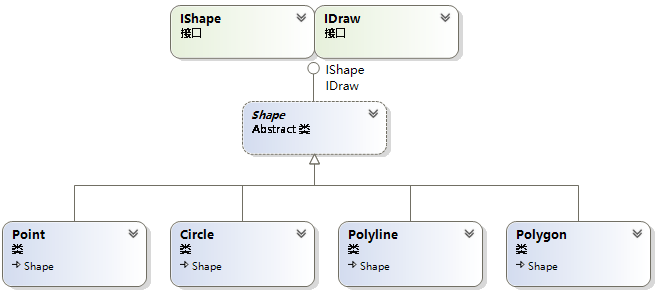
\includegraphics[scale=0.6]{chapter/csobject/graph.png}
	\caption{几何图形关系类图}
	\label{fig:graph}
\end{figure}

请注意,类图\ref{fig:graph} 中所有的类均用实线矩形表示。

我们首先将所有图形对象的公有属性面积 Area、长度Length 和 计算 Calculate、绘图 Draw 方法抽象到基类 Shape中,代码如下:

\begin{lstlisting}
public class Shape
{
	protected double length = 0.0;
	public double Length { get => length; }
	
	protected double area = 0.0;
	public double Area { get =>area; }
	
	public virtual void Calculate() { }
	public virtual void Draw()
	{
		Console.WriteLine("Shape Draw ......");
	}
}
\end{lstlisting}

由于各种图形计算长度与面积的方法各不相同,所以将 Calculate() 方法与 Draw() 方法定义为虚函数virtual(), Calculate() 方法采用默认的空函数体方式实现;
length与area用于存储各种图形的计算值,要求外部对象不能访问与修改,定义为受保护权限(protected),通过只读属性向外部展现数据。

点类 Point 的实现如下:

\begin{lstlisting}
public class Point : Shape
{      
	public double X { get; set; }
	public double Y { get; set; }        
	
	public Point(double x, double y)
	{          
		this.X = x;
		this.Y = y;          
	}
	
	public override void Draw()
	{
		Console.WriteLine("Point Draw ......");
	}
}
\end{lstlisting}

点Point的面积与长度我们均默认为 0, Shape类中的计算功能就够了,此处就不在覆盖(override);绘图需要修改为 ``Point Draw ... '' 形式,故需覆盖(override)。

圆类 Circle 的实现如下:

\begin{lstlisting}
public class Circle : Shape
{
	public Point Center { get; set; }
	
	private double r;
	public double R
	{
		get { return r; }
		set
		{
			if(value != r && value >= 0)
			{
				r = value;
				Calculate(); //r的值发生改变,重新计算圆的面积
			}
		}
	}
	
	
	public Circle(double x, double y, double r)
	{
		Center = new Point(x, y);
		this.R = r;  //赋值给R而不是this.r,确保计算圆的面积
	}
	
	public override void Calculate()
	{
		this.length = Math.PI * r * 2;
		this.area = Math.PI * r * r;
		
	}
	
	public override void Draw()
	{
		Console.WriteLine("Circle Draw ......");
	}
}
\end{lstlisting}

由于圆类的面积与周长计算方法与基类Shape不同,需将 Calculate() 与 Draw() 方法覆盖(override)。




多段线类 Polyline 的实现如下:

\begin{lstlisting}
public class Polyline : Shape
{
	private List<Point> points = new List<Point>();
	
	private double CalLength()
	{
		if (points.Count < 2) return 0;
		double sum = 0;
		for (int i = 0; i < points.Count - 1; i++)
		{
			double dx = points[i + 1].X - points[i].X;
			double dy = points[i + 1].Y - points[i].Y;
			sum += Math.Sqrt(dx * dx + dy * dy);
		}
		return sum;
	}       
	
	public void Add(double x, double y)
	{
		points.Add(new Point(x, y));
	}
	
	public Polyline()
	{
	}       
	
	public override void Calculate()
	{
		this.length = CalLength();
		this.area = 0.0;
		
	}
	
	public override void Draw()
	{
		Console.WriteLine("Polyline Draw ......");
	}
}
\end{lstlisting}

由于多段线类的面积与周长计算方法与基类Shape不同,需将 Calculate() 与 Draw() 方法覆盖(override)。


多边形类 Polygone 的实现如下:

\begin{lstlisting}
public class Polygon : Shape
{
	private List<Point> points = new List<Point>();
	
	public double CalLength()
	{
		if (points.Count < 2) return 0;
		double sum = 0;
		for (int i = 0; i < points.Count; i++)
		{
			int j = (i + 1) % points.Count;
			double dx = points[j].X - points[i].X;
			double dy = points[j].Y - points[i].Y;
			sum += Math.Sqrt(dx * dx + dy * dy);
		}
		return sum;
	}
	
	public double CalArea()
	{
		if (points.Count < 3) return 0;
		double s = 0;
		for (int i = 0; i < points.Count; i++)
		{
			int j = i + 1;
			if (j == points.Count) j = 0;
			s += points[i].X * points[j].Y - points[j].X * points[i].Y;
		}
		return 0.5 * Math.Abs(s);
	}
	
	public void Add(double x, double y)
	{
		points.Add(new Point(x, y));
	}
	
	public override void Calculate()
	{
		this.length = CalLength();
		this.area = CalArea();
		
	}
	
	public override void Draw()
	{
		Console.WriteLine("Polygon Draw ......");
	}
}
\end{lstlisting}

由于多边形类的面积与周长计算方法与基类Shape不同,需将 Calculate() 与 Draw() 方法覆盖(override)。

客户端调用的代码如下:
\begin{lstlisting}
class Program
{
	static void Main(string[] args)
	{
		Shape s = new Shape();
		s.Calculate();
		Console.WriteLine("Shape's Area={0}, Length={1}", s.Area, s.Length);
		s.Draw();
		
		Point p = new Point(100, 100);
		p.Calculate();
		Console.WriteLine("Point's Area={0}, Length={1}", p.Area, p.Length);
		p.Draw();
		
		Circle c = new Circle(100, 100, 80);
		c.Calculate();
		Console.WriteLine("Circle1's Area={0}, Length={1}", c.Area, c.Length);
		c.Draw();
		
		Polyline pl = new Polyline();
		pl.Add(-1, 0);
		pl.Add(2, 3);
		pl.Add(4, 2);
		pl.Add(4, 4);
		pl.Add(6, 8);
		pl.Add(-2, 5);
		pl.Calculate();
		Console.WriteLine("Polyline's Area={0}, Length={1}", pl.Area, pl.Length);
		pl.Draw();
		
		Polygon pg = new Polygon();
		pg.Add(-1, 0);
		pg.Add(2, 3);
		pg.Add(4, 2);
		pg.Add(4, 4);
		pg.Add(6, 8);
		pg.Add(-2, 5);
		pg.Calculate();
		Console.WriteLine("Polygon's Area={0}, Length={1}", pg.Area, pg.Length);
		pg.Draw();
		
		Console.ReadKey();
	}
}
\end{lstlisting}

代码运行输出为:

\begin{verbatim}
Shape's Area=0, Length=0
Shape Draw ......
Point's Area=0, Length=0
Point Draw ......
Circle1's Area=20106.1929829747, Length=502.654824574367
Circle Draw ......
Polyline's Area=0, Length=21.4948483649362
Polyline Draw ......
Polygon's Area=28, Length=26.593867878529
Polygon Draw ......	
\end{verbatim}

很明显,客户端的调用代码有问题,如果增加一个图形实例的,调用代码就需要增加,代码会无限膨胀,对于绘图程序,也无法统一在屏幕上进行绘制与计算。更加合理的客户端调用的代码如下所示:

\begin{lstlisting}
class Program
{
	static void Main(string[] args)
	{
		List<Shape> shapeList = new List<Shape>();
		shapeList.Add(new Shape());
		shapeList.Add(new Point(100, 100));
		shapeList.Add(new Circle(100, 100, 80));
		
		Polyline pl = new Polyline();
		pl.Add(-1, 0);
		pl.Add(2, 3);
		pl.Add(4, 2);
		pl.Add(4, 4);
		pl.Add(6, 8);
		pl.Add(-2, 5);
		shapeList.Add(pl);
		
		Polygon pg = new Polygon();
		pg.Add(-1, 0);
		pg.Add(2, 3);
		pg.Add(4, 2);
		pg.Add(4, 4);
		pg.Add(6, 8);
		pg.Add(-2, 5);
		shapeList.Add(pg);
		
		CalculateAll(shapeList);
		DrawAll(shapeList);
		
		
		Console.ReadKey();
	}
		
	static void CalculateAll(List<Shape> shapeList)
	{
		foreach (var item in shapeList)
		{
			item.Calculate();
			Console.WriteLine("Area={0}, Length={1}", item.Area, item.Length);               
		}
	}
		
	static void DrawAll(List<Shape> shapeList)
	{
		foreach (var item in shapeList)
		{
			item.Draw();
		}
	}
}
\end{lstlisting}

代码运行输出为:

\begin{verbatim}
Area=0, Length=0
Area=0, Length=0
Area=20106.1929829747, Length=502.654824574367
Area=0, Length=21.4948483649362
Area=28, Length=26.593867878529
Shape Draw ......
Point Draw ......
Circle Draw ......
Polyline Draw ......
Polygon Draw ......
\end{verbatim}

这样写的好处是28-50行的代码基本稳定,图形实例的增加不会再去修改这部分代码。

可能有人认为这次的面积与长度输出看不到图形信息,其实对各个类的 ToString 函数覆盖(override)就可以达到与前面一样的效果,代码如下:
\begin{lstlisting}
public class Shape
{
 	........................
	
	public override string ToString()
	{
		return $"Shape's Area ={Area}, Length ={Length}";
	}
}

public class Point : Shape
{      
 	........................
	
	public override string ToString()
	{
		return $"Point's Area ={Area}, Length ={Length}";
	}
}

public class Circle : Shape
{
	........................
	
	public override string ToString()
	{
		return $"Circle's Area ={Area}, Length ={Length}";
	}
}

public class Polyline : Shape
{
	........................
		
	public override string ToString()
	{
		return $"Polyline's Area ={Area}, Length ={Length}";
	}
}

public class Polygon : Shape
{
	........................
	 
	public override string ToString()
	{
		return $"Polygon's Area ={Area}, Length ={Length}";
	}
}

\end{lstlisting}

ToString() 函数来自 System.Object 类, System.Object 类是所有的类的根, ToString() 函数被定义为 virtual。

CalculateAll函数稍作修改:
\begin{lstlisting}
static void CalculateAll(List<Shape> shapeList)
{
	foreach (var item in shapeList)
	{
		item.Calculate();
		Console.WriteLine(item);               
	}
}	
\end{lstlisting}

则运行输出结果为:
\begin{verbatim}
Shape's Area =0, Length =0
Point's Area =0, Length =0
Circle's Area =20106.1929829747, Length =502.654824574367
Polyline's Area =0, Length =21.4948483649362
Polygon's Area =28, Length =26.593867878529
Shape Draw ......
Point Draw ......
Circle Draw ......
Polyline Draw ......
Polygon Draw ......
\end{verbatim}


\section{抽象方法与抽象类}

在上节的内容中,Shape类的虚函数Calculate函数体为空,什么内容都不做;在实际的绘图成图中,Draw函数也一样。
因此可以用关键字 abstract 将其定义为抽象方法,就可以不定义函数体了。

含有一个抽象方法的类就是抽象类,必须在关键字 class 前用 abstract 加以定义,抽象类 Shape 代码如下所示:

\begin{lstlisting}
public abstract class Shape
{
	protected double length = 0.0;
	public double Length { get => length; }
	
	protected double area = 0.0;
	public double Area { get =>area; }
	
	public abstract void Calculate();
	public abstract void Draw();
}
\end{lstlisting}

抽象类不同于普通实例类的特点是不能实例化,不能写成: \verb|Shape s = new Shape()|,但可以写成
\verb|Shape s = new Point()| 形式。

抽象方法不同于虚函数的地方在于派生类中必须覆盖(override)抽象方法,而虚函数则没有这样强制性的要求。
因此前面的Point类由于没有覆盖(override) 基类Shape中的抽象方法 Calculate,需做如下修改:

\begin{lstlisting}
public sealed class Point : Shape
{      
	........................
	
	public override void Draw()
	{
		Console.WriteLine("Point Draw ......");
	}
	
	........................
}
\end{lstlisting}


在类图中,抽象类是用虚线矩形表示的,如图 \ref{fig:agraph} 所示:
\begin{figure}[htbp]
	\centering
	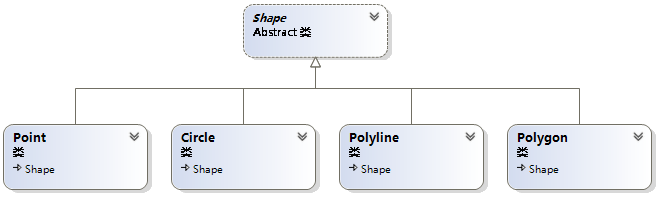
\includegraphics[scale=0.6]{chapter/csobject/agraph.png}
	\caption{几何图形关系类图的抽象类}
	\label{fig:agraph}
\end{figure}

由于抽象类Shape不能实例化,前面的调用代码中生成Shape实例的代码需删除,如下代码所示:
\begin{lstlisting}
class Program
{
	static void Main(string[] args)
	{		
		List<Shape> shapeList = new List<Shape>();
		//shapeList.Add(new Shape()); //需删除
		shapeList.Add(new Point(100, 100));
		shapeList.Add(new Circle(100, 100, 80));
		
		........................
	}
	
	........................
}
\end{lstlisting}




\section{接口(interface)}
接口是指公开约定的属性或方法,接口是面向对象编程方法的重要概念。

接口的关键字是 interface, 与抽象类不同的是接口中只能含有方法与属性,所有的方法与属性均不能有具体的实现。

\begin{figure}[htbp]
	\centering
	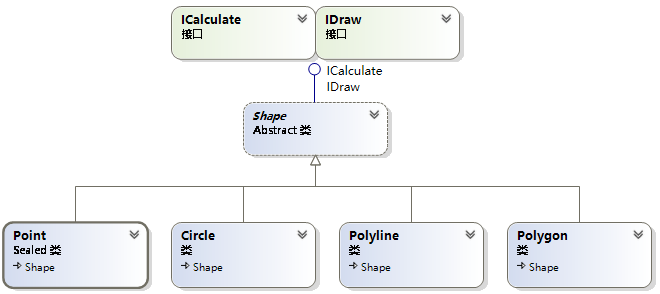
\includegraphics[scale=0.6]{chapter/csobject/igraph.png}
	\caption{带有接口的几何图形关系类图}
	\label{fig:igraph}
\end{figure}

如图 \ref{fig:igraph}所示,我们设计图形接口IShape与绘制接口ICalculate :

\begin{lstlisting}
public interface ICalculate
{
	void Calculate();
}

public interface IDraw
{
	void Draw();
}
\end{lstlisting}

让抽象类 Shape 来实现这两个接口:

\begin{lstlisting}
public abstract class Shape : ICalculate, IDraw
{
	protected double length = 0.0;
	public double Length { get => length; }
	
	protected double area = 0.0;
	public double Area { get =>area; }
	
	public abstract void Calculate();
	public abstract void Draw();
}
\end{lstlisting}

实现接口也可以用一般的实例类,也可以用一般的方法,也可以用虚函数,也可以抽象方法,只要方法的签名与接口相符就行。

在我们的这个例子中,我们使用抽象类的抽象函数进行接口实现。

\subsection{面向接口编程}

接口是框架系统设计的关键技术,众多的商业软件为了易于扩展与修改,也为了多人协调开发,均是以架构形式出现,系统架构师的主要设计手段就是面向接口进行设计与编码。有兴趣的同学可以研读设计模式等相关资料。

在我们的例子中,如下代码中的CalculateAll与DrawAll函数分别是面向接口ICalculate与IDraw接口编写的:

\begin{lstlisting}
class Program
{
	static void Main(string[] args)
	{		
		List<Shape> shapeList = new List<Shape>();
		shapeList.Add(new Point(100, 100));
		shapeList.Add(new Circle(100, 100, 80));
		
		Polyline pl = new Polyline();
		pl.Add(-1, 0);
		pl.Add(2, 3);
		pl.Add(4, 2);
		pl.Add(4, 4);
		pl.Add(6, 8);
		pl.Add(-2, 5);
		shapeList.Add(pl);
		
		Polygon pg = new Polygon();
		pg.Add(-1, 0);
		pg.Add(2, 3);
		pg.Add(4, 2);
		pg.Add(4, 4);
		pg.Add(6, 8);
		pg.Add(-2, 5);
		shapeList.Add(pg);
		
		List<IDraw> drawList = new List<IDraw>();
		foreach (var item in shapeList)
		{
			IDraw idraw = item;
			drawList.Add(idraw);
		}
		DrawAll(drawList);
		
		List<ICalculate> calculateList = new List<ICalculate>();
		foreach (var item in calculateList)
		{
			ICalculate icalculate = item as ICalculate;
			calculateList.Add(icalculate);
		}
		CalculateAll(calculateList);
		
		foreach (var item in shapeList)
		{                
			Console.WriteLine(item);
		}
		
		Console.ReadKey();
	}
		
	static void CalculateAll(List<ICalculate> calculateList)
	{
		foreach (var item in calculateList)
		{
			item.Calculate();           
		}
	}
		
	static void DrawAll(List<IDraw> shapeList)
	{
		foreach (var item in shapeList)
		{
			item.Draw();
		}
	}
}
\end{lstlisting}

代码中第27-32行是用接口IDraw指向各个Shape实例,以满足DrawAll的接口调用要求。


\subsection{接口跳转}

在某些软件设计中,有将某个类设计的功能特别多的情况,就可以用接口将这些功能分组,在使用的时候,某个接口功能使用完毕,就可以进行接口跳转,再去使用其他功能。

在上面的代码第38行:
\verb|ICalculate icalculate = item as ICalculate;| 就是从接口 IDraw 跳转到 ICalculate。

这种跳转之所以能成功,是因为这些接口所指向的实例对象均实现了这些接口,否则,这种跳转将失败。


\section{封闭类(sealed class)}

如果一个类不需要再通过继承扩展,就可以用关键字 sealed 将其定义为封闭类,比如点Point类:
\begin{lstlisting}
public sealed class Point : Shape
{      
	public double X { get; set; }
	public double Y { get; set; }        
	
	public Point(double x, double y)
	{          
		this.X = x;
		this.Y = y;          
	}
	
	public override void Calculate()
	{
		this.area = 0.0;
		this.length = 0.0;
	}
	
	public override void Draw()
	{
		Console.WriteLine("Point Draw ......");
	}
	
	public override string ToString()
	{
		return $"Point's Area ={Area}, Length ={Length}";
	}
}
\end{lstlisting}

\section{小结}

多态的实现条件是这些类要满足继承关系,也就是多态只能发生在基类与派生类之间;

要实现多态,需将基类的方法定义为虚函数(virtual),派生类根据需要覆盖(override)相应的基类虚函数;

抽象方法不需要函数体,含有一个抽象方法的类必须定义为抽象类,抽象类不能实例化;

接口中不能含有字段,只能有方法与属性,接口可以继承接口,接口支持多继承,继承自接口的类必须实现接口。